%!TEX root = ../main.tex

\section{Results and discussion}

This section provides results and related discussions for modeling the effects of different fluidization gases on the operation of a bubbling fluidized bed reactor. Gas effects on the pyrolysis yields of the biomass feedstock are also presented and discussed.

% ----------------------------------------------------------------------------

\subsection{Pure gas properties}

Molecular weight, viscosity, density, thermal conductivity, heat capacity, and the Prandtl number of the individual gases investigated in this paper are shown in Figure \ref{fig:gas-properties}. The gas properties were calculated at a pressure of 101,325 Pa and a temperature of 773.15 K (500$^\circ$C). The lightest gas in terms of molecular weight and density is hydrogen while the heaviest gas is carbon dioxide. The highest viscosity is noted for the nitrogen gas while hydrogen has the lowest viscosity. The largest thermal conductivity is for hydrogen at approximately 0.36 W/(m\,K) while the other gases remain below 0.12 W/(m\,K). The highest heat capacity is obtained for methane at 62 J/(mol\,K) while the lowest is for hydrogen at 29 J/(mol\,K). The Prandtl number is similar for all the gases except for water vapor.

\begin{figure}[H]
    \centering
    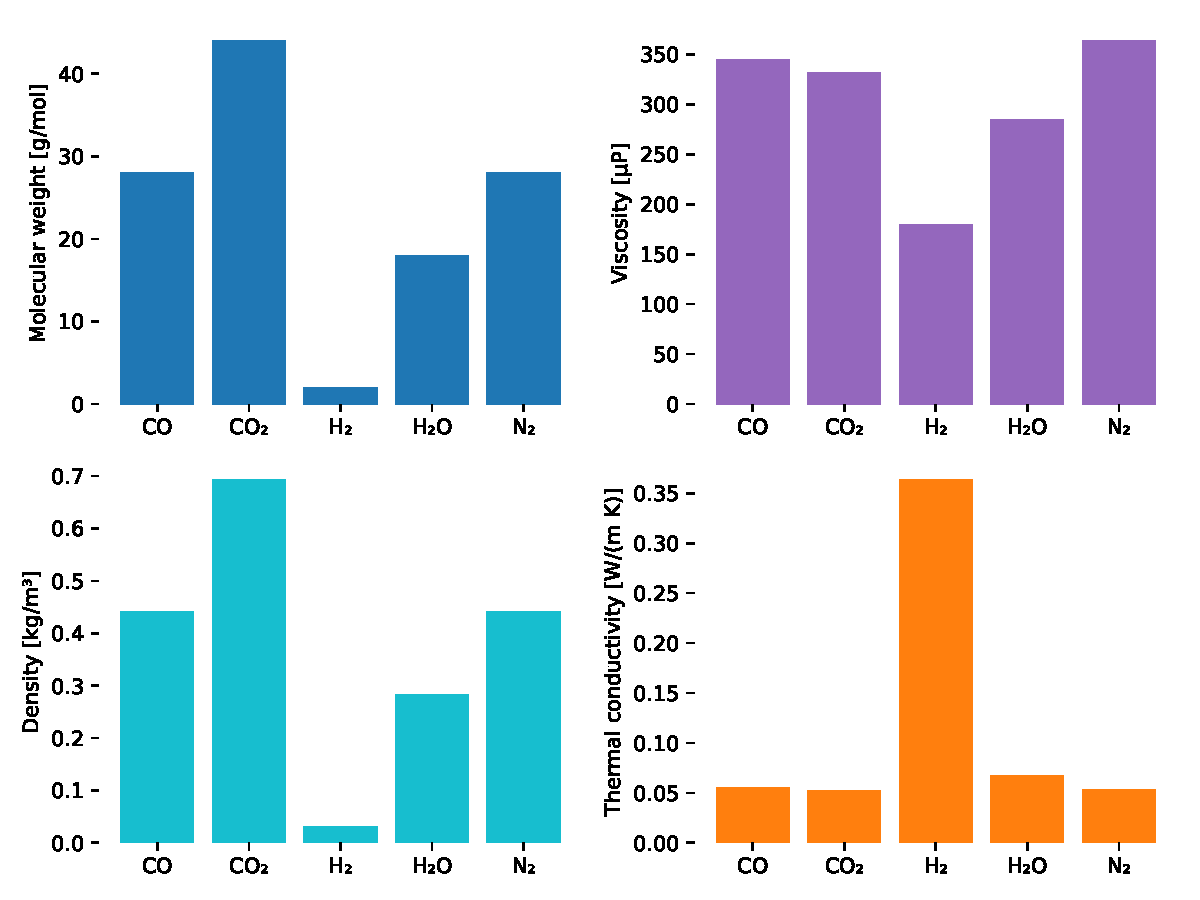
\includegraphics[width=\textwidth]{gas-properties.pdf}
    \caption{Comparison of molecular weight (MW), viscosity ($\mu$), density ($\rho$), thermal conductivity (k), heat capacity (Cp), and Prandtl number (Pr) for each gas at 101,325 Pa and 773.15 K (500$^\circ$C).}
    \label{fig:gas-properties}
\end{figure}

% ----------------------------------------------------------------------------

\subsection{Gas mixture properties}

Comparisons of the calculated viscosity of a H$_2$/N$_2$ gas mixture to measured values obtained from literature are shown in Figure \ref{fig:gas-mu-h2n2-validate}. The models by Herning and Zipperer as well as Brokaw match well with the experimental data for a range of mixture ratios. This is contradictory to the Davidson report which does not recommend the Herning and Zipperer model for hydrogen mixtures \cite{Davidson-1993}. The Davidson and Graham models significantly underpredict the mixture viscosity while the Wilke model tends to overestimate the viscosity. Similar results are obtained for a H$_2$/O$_2$ gas mixture as shown in Figure \ref{fig:gas-mu-h2o2-validate}.

\begin{figure}[H]
    \centering
    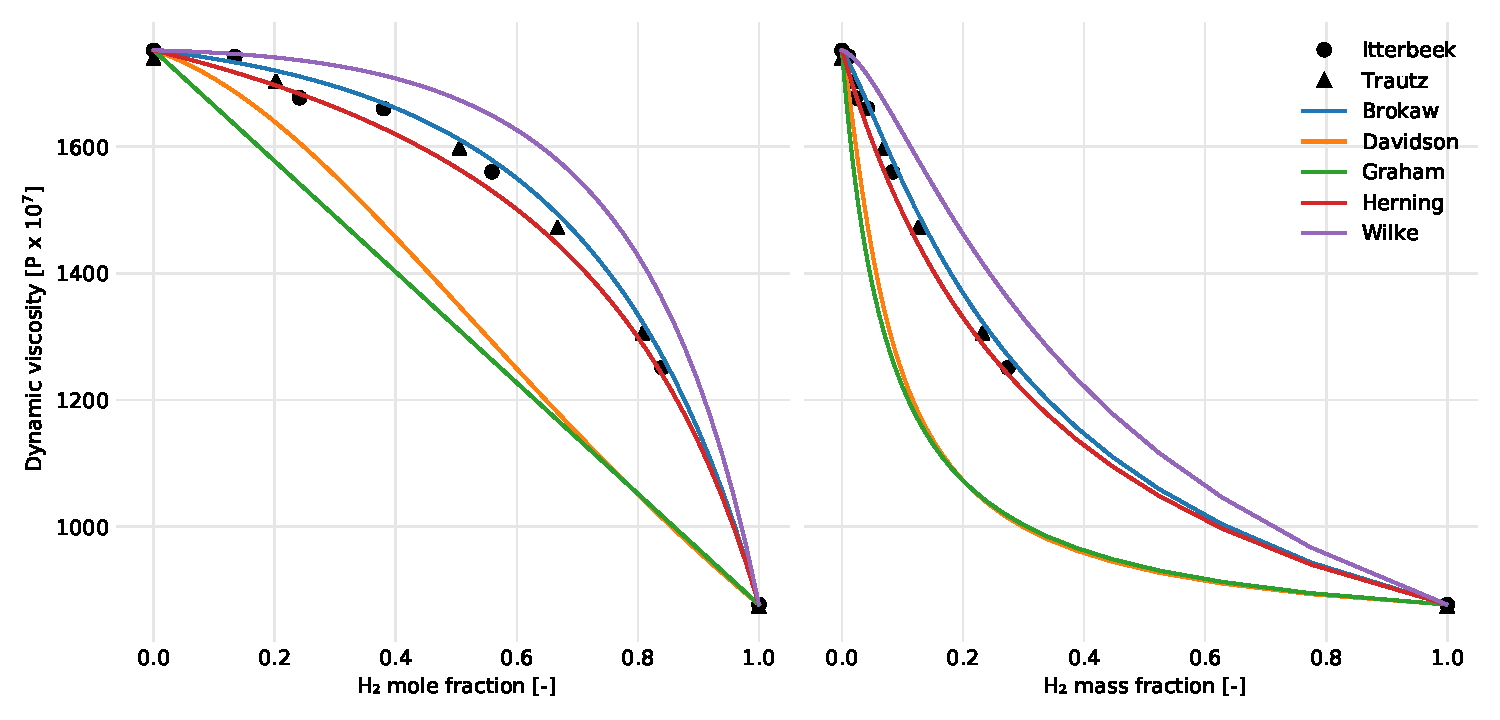
\includegraphics[width=\textwidth]{figures/gas-mu-h2n2-validate.pdf}
    \caption{Viscosity of a H$_2$/N$_2$ mixture at 291.1 K (18$^\circ$C). Calculated values represented by line profiles. Experiment data points from \cite{Itterbeek-1947,Trautz-1929} shown as symbols.}
    \label{fig:gas-mu-h2n2-validate}
\end{figure}

\begin{figure}[H]
    \centering
    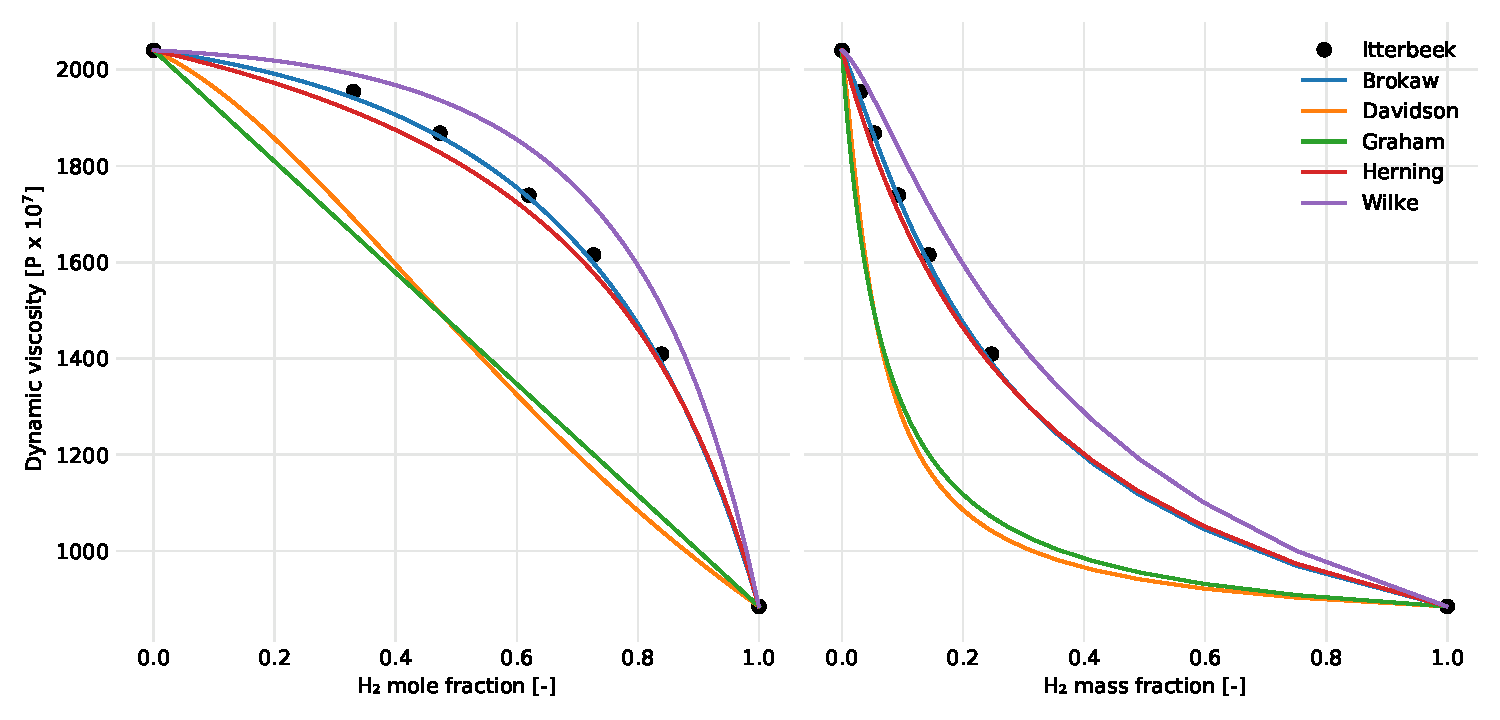
\includegraphics[width=\textwidth]{figures/gas-mu-h2o2-validate.pdf}
    \caption{Viscosity of a H$_2$/O$_2$ mixture at 293.6 K (20$^\circ$C). Calculated values represented by line profiles. Experiment data points from \cite{Itterbeek-1947} shown as symbols.}
    \label{fig:gas-mu-h2o2-validate}
\end{figure}

Properties for molecular weight, viscosity, and density for the gas mixtures investigated in this paper are shown in Figure \ref{fig:mix-properties}. Similar to the individual gas properties, the mixture properties were calculated at 101,325 Pa and 773.15 K (500$^\circ$C). The fraction of each gas in the mixture is given by the values shown at the top of each column in the figure. For example, the hydrogen and nitrogen mixture is comprised of 80\% hydrogen and 20\% nitrogen which is labeled as $0.8 + 0.2$. As expected, the carbon dioxide mixture is the heaviest in terms of molecular weight and density.

\begin{figure}[H]
    \centering
    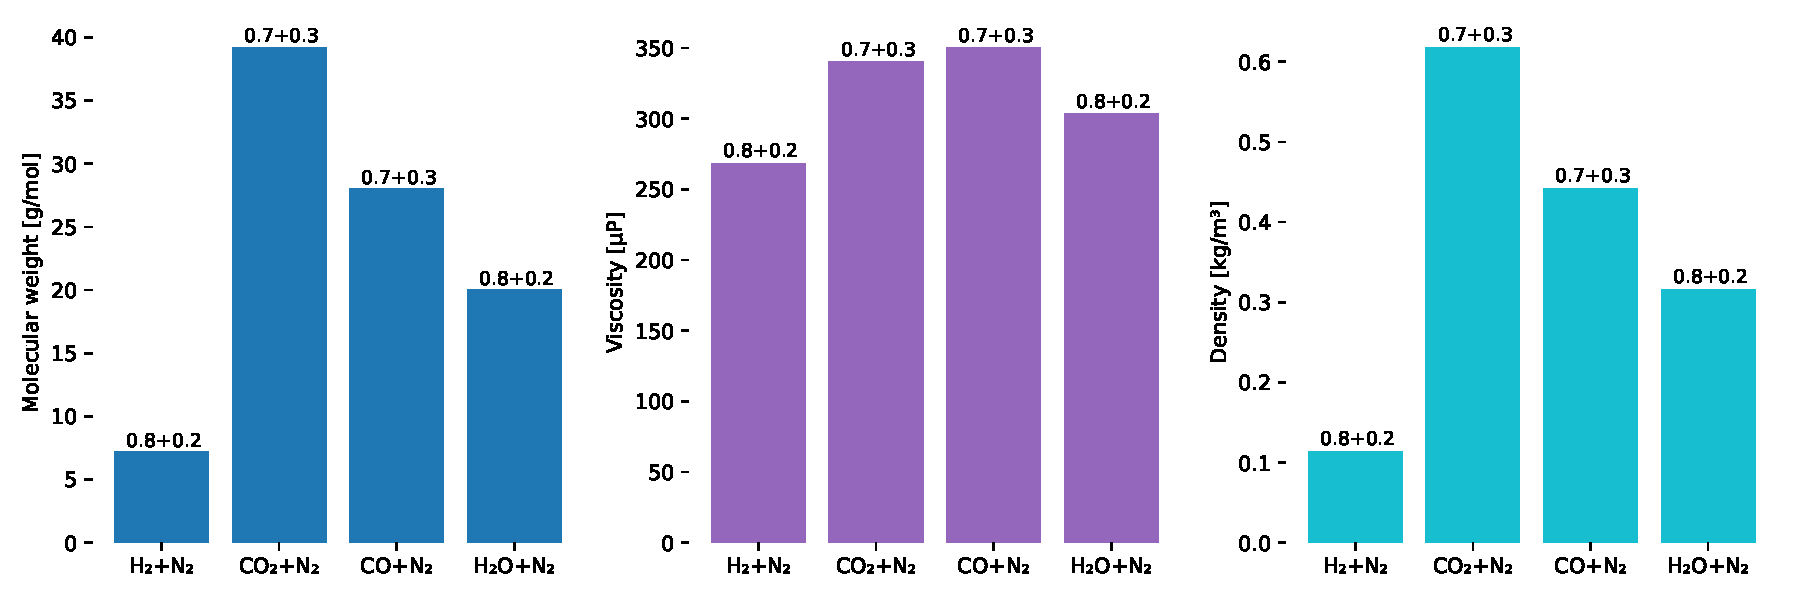
\includegraphics[width=\textwidth]{mix-properties.pdf}
    \caption{Comparison of gas mixture properties for molecular weight, viscosity, and density at 101,325 Pa and 773.15 K. Fraction of each gas component is shown at the top of each column.}
    \label{fig:mix-properties}
\end{figure}

% ----------------------------------------------------------------------------

\subsection{Fluidization characteristics}

Minimum fluidization velocity (U$_\text{mf}$) of the bed material for the different fluidization gases is presented in Table \ref{tab:umf-sand}. Hydrogen requires about twice the gas velocity to fluidize the bed of sand compared to the nitrogen, carbon monoxide, and carbon dioxide gases. This is due to hydrogen's lower viscosity and much lower density compared to the other gases. Water vapor and methane require moderately higher fluidization velocities compared to the nitrogen gas. A comparison of U$_\text{mf}$ for the various fluidization gases is displayed in Figure \ref{fig:umf-usumf-gases}.

\begin{table}[H]
    \centering
    \caption{Minimum fluidization velocity (m/s) of the bed material calculated from various correlations for different fluidization gases. Last row represents the average U$_\text{mf}$ value for each gas.}
    \label{tab:umf-sand}
    \begin{tabular}{lrrrrrr}
        \toprule
        U$_\text{mf}$ & N$_2$ & H$_2$ & H$_2$O & CO & CO$_2$ & CH$_4$ \\
        \midrule
        Ergun         & 0.14 & 0.30 & 0.18 & 0.15 & 0.16 & 0.23 \\
        Grace         & 0.10 & 0.21 & 0.13 & 0.11 & 0.11 & 0.16 \\
        Richardson    & 0.10 & 0.20 & 0.12 & 0.10 & 0.11 & 0.15 \\
        Wen and Yu    & 0.08 & 0.17 & 0.11 & 0.09 & 0.09 & 0.13 \\
        average       & 0.11 & 0.22 & 0.14 & 0.11 & 0.12 & 0.17 \\
        \bottomrule
    \end{tabular}
\end{table}

The superficial gas velocity (U$_\text{s}$) of the nitrogen gas flow is calculated as 0.3072 m/s which is based on the 14 SLM gas flow through the distributor plate. Using this value, the ratio of U$_\text{s}$ to U$_\text{mf}$ is shown in Table \ref{tab:us-umf-ratio} for different fluidization gases. The BFB pyrolysis reactor at NREL typically operates at a U$_\text{s}$/U$_\text{mf}$ of 3 with nitrogen gas. For gases such as H$_2$, H$_2$O, CO, CO$_2$, and CH$_4$, the gas flow into the reactor must be increased to have similar fluidized bed characteristics as the nitrogen case. A comparison of the increased U$_\text{s}$ for each gas along with the associated U$_\text{s}$/U$_\text{mf}$ is shown in Figure \ref{fig:us-usumf-gases}. As expected, the hydrogen gas flow must be approximately doubled compared to the nitrogen case to achieve similar fluidization of the bed material.

\begin{table}[H]
    \centering
    \caption{Ratio of U$_\text{s}$ to U$_\text{mf}$ for different fluidization gases. Last row represents the average U$_\text{s}$/U$_\text{mf}$ value for each gas.}
    \label{tab:us-umf-ratio}
    \begin{tabular}{lrrrrrr}
        \toprule
        U$_\text{s}$/U$_\text{mf}$ & N$_2$ & H$_2$ & H$_2$O & CO & CO$_2$ & CH$_4$ \\
        \midrule
        Ergun                      & 2.13 & 1.04 & 1.67 & 2.02 & 1.97 & 1.34 \\
        Grace                      & 2.99 & 1.47 & 2.35 & 2.84 & 2.76 & 1.88 \\
        Richardson                 & 3.16 & 1.55 & 2.48 & 3.00 & 2.91 & 1.98 \\
        Wen and Yu                 & 3.69 & 1.82 & 2.90 & 3.50 & 3.39 & 2.32 \\
        average                    & 2.99 & 1.47 & 2.35 & 2.84 & 2.76 & 1.88 \\
        \bottomrule
    \end{tabular}
\end{table}

\begin{figure}[H]
    \centering
    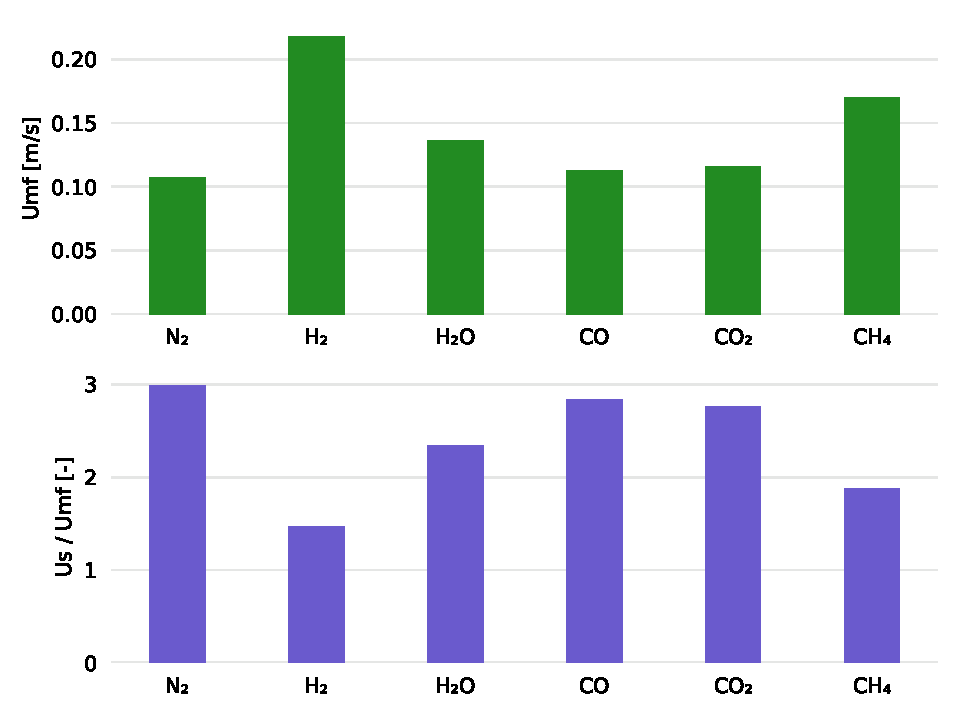
\includegraphics[width=0.8\textwidth]{figures/umf-usumf-gases.pdf}
    \caption{Comparison of the minimum fluidization velocity (U$_\text{mf}$) and the ratio of U$_\text{s}$/U$_\text{mf}$ for different fluidization gases. Superficial gas velocity is U$_\text{s}$.}
    \label{fig:umf-usumf-gases}
\end{figure}

\begin{figure}[H]
    \centering
    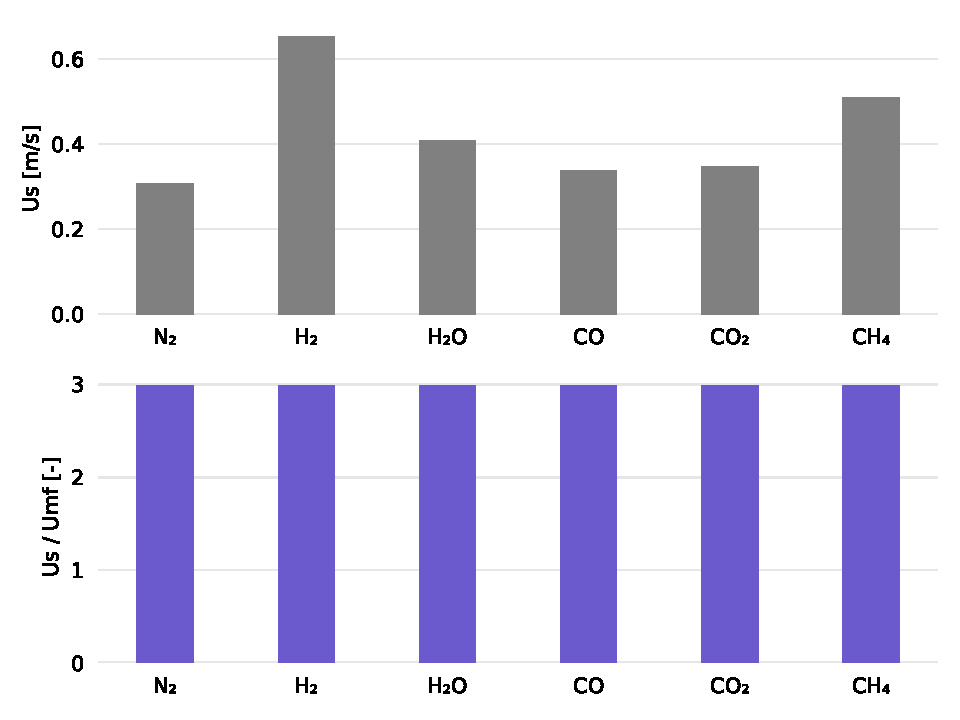
\includegraphics[width=0.8\textwidth]{figures/us-usumf-gases.pdf}
    \caption{Comparison of the superficial gas velocity (U$_\text{s}$) and the associated U$_\text{s}$/U$_\text{mf}$ for different fluidization gases. Minimum fluidization velocity is U$_\text{mf}$.}
    \label{fig:us-usumf-gases}
\end{figure}

The Reynolds number was calculated using an average biomass particle diameter of 369.4 $\mu$m and the mean U$_\text{mf}$ value. Next, the Nusselt number along with the associated convective heat transfer coefficient were calculated for each carrier gas as shown in Table \ref{tab:biomass-hconv} and Figure \ref{fig:biomass-hconv}. The highest heat transfer coefficient is estimated for H$_2$ while the second highest result is for CH$_4$. This is largely due to the higher thermal conductivity of the hydrogen and methane compared to the other gases. Due to the higher heat transfer rate to the biomass particle in the hydrogen environment, one can expect the biomass to pyrolyze more quickly with the hydrogen carrier gas.

\begin{table}[H]
    \centering
    \caption{Comparison of the Reynolds number, Nusselt number, and convective heat transfer coefficient (h) for different fluidization gases.}
    \label{tab:biomass-hconv}
    \begin{tabular}{lrrrr}
        \toprule
        Gas & U$_\text{mf}$ & Re & Nu & h \\
        \midrule
        N$_2$  & 0.11 & 0.48 & 2.55 & 369.45  \\
        H$_2$  & 0.22 & 0.14 & 2.26 & 2224.25 \\
        H$_2$O & 0.14 & 0.50 & 2.56 & 464.54  \\
        CO     & 0.11 & 0.53 & 2.58 & 389.53  \\
        CO$_2$ & 0.12 & 0.89 & 2.81 & 399.83  \\
        CH$_4$ & 0.17 & 0.70 & 2.69 & 862.61  \\
        \bottomrule
    \end{tabular}
\end{table}

\begin{figure}[H]
    \centering
    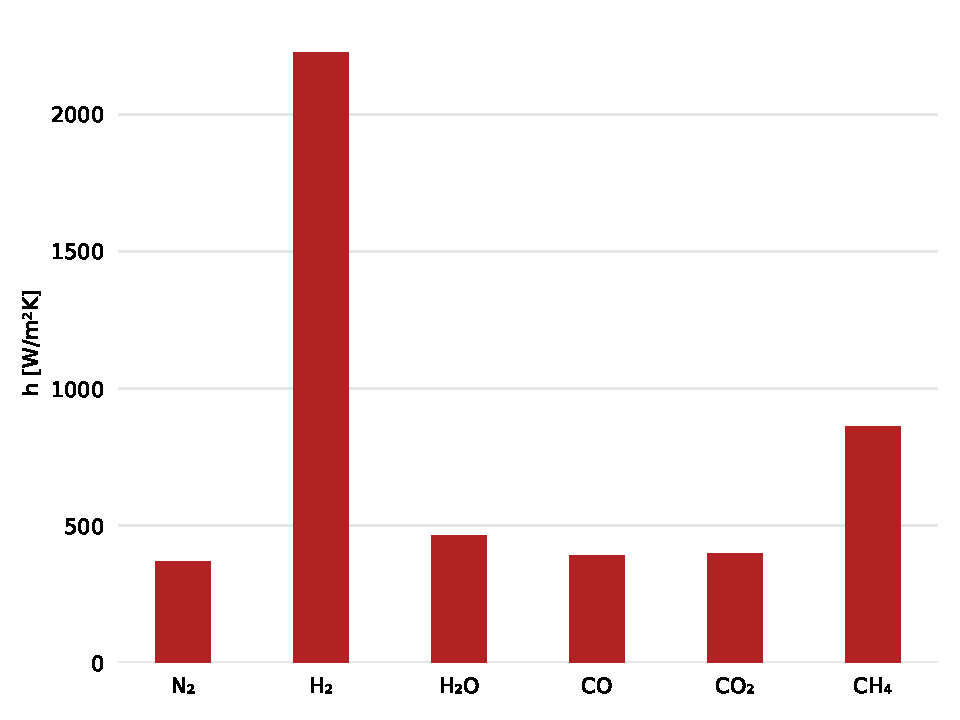
\includegraphics[width=0.8\textwidth]{figures/biomass_hconv.pdf}
    \caption{Convective heat transfer coefficient (h) for different fluidization gases. Values based on average biomass particle size and average minimum fluidization velocity.}
    \label{fig:biomass-hconv}
\end{figure}

% ----------------------------------------------------------------------------

\subsection{Evaluation of the kinetic scheme}

The Di Blasi kinetics were put to use in a batch reactor model to investigate the time scales associated with the reaction mechanisms. Figure \ref{fig:batch-blasi} is an overview of the biomass conversion and product yields using the Di Blasi kinetics in a batch reactor at 773.15 K (500$^\circ$C). At this temperature, without the effects of secondary reactions, the kinetics offer a maximum achievable tar yield of 78\% within 5 seconds. However, if secondary reactions occur during the entire pyrolysis process then a maximum tar yield of only 53\% is possible. The Di Blasi kinetics suggest that minimizing the extent of secondary reactions is critical to producing the maximum possible tar yield.

A range of reaction temperatures were applied to the Di Blasi kinetics in the batch reactor model as shown in Figure \ref{fig:batch-blasi-temps}. The kinetics suggest that temperature has a neglible effect on primary tar yield but effects of secondary reactions are more pronounced. When secondary reactions occur during the entire pyrolysis process, maximum tar yields are realized at higher temperatures but with shorter residence times. These results suggest that if secondary reactions are minimized then temperature should not have a drastic effect on tar yield.

\begin{figure}[H]
    \centering
    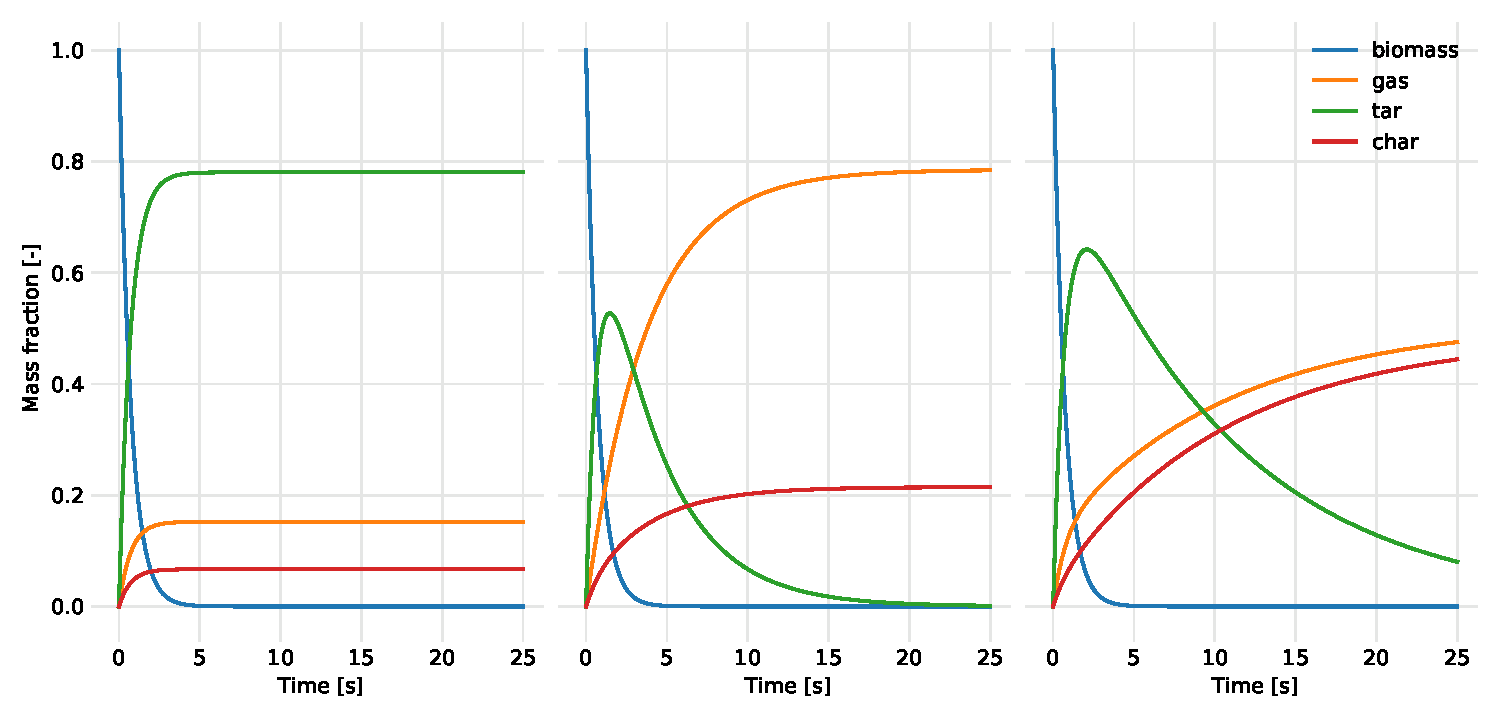
\includegraphics[width=\textwidth]{batch-blasi.pdf}
    \caption{Biomass conversion and product yields in a batch reactor model at 773.15 K (500$^\circ$C) according to the Di Blasi kinetic reactions. Primary reactions only (left). Primary and secondary reactions (center). Primary and secondary reactions using modified reaction 4 (right).}
    \label{fig:batch-blasi}
\end{figure}

\begin{figure}[H]
    \centering
    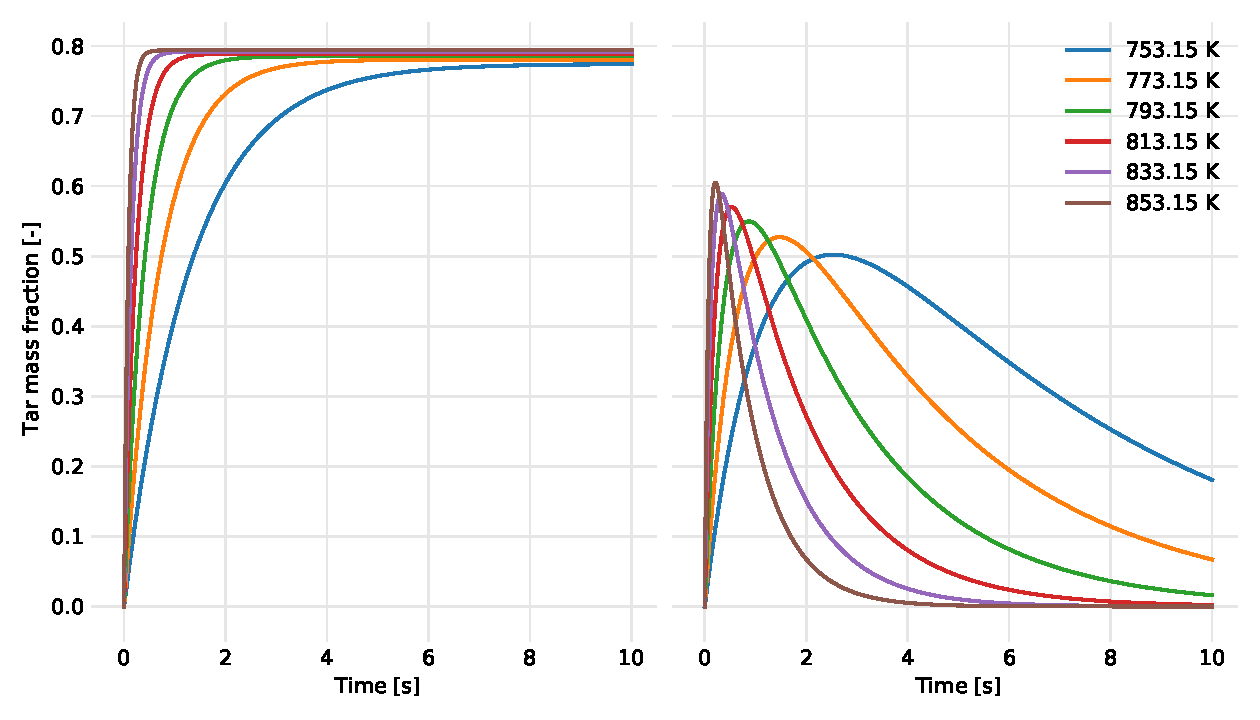
\includegraphics[width=\textwidth]{batch-blasi-temps.pdf}
    \caption{Tar yields for reaction temperatures of 753.15--853.15 K (480--580$^\circ$C) using the Di Blasi kinetics in a batch reactor model. Results shown for primary tar (left) along with primary and secondary tar (right).}
    \label{fig:batch-blasi-temps}
\end{figure}

% ----------------------------------------------------------------------------

\subsection{Limiting factors for biomass pyrolysis}

Gas influence on the pyrolysis limiting regimes is shown in Figure \ref{fig:biot-pyro-gases} for a biomass particle diameter of 369.4 $\mu$m. The regime map suggests that gas properties have little effect on the limiting mode of pyrolysis. However, when comparing a range of particle diameters, the differences are more pronounced as seen in Figure \ref{fig:biot-pyro-diams}. For larger particles, conduction becomes the limiting mode of pyrolysis especially for the hydrogen gas. For smaller particles, nitrogen gas promotes isothermal conditions along with a kinetically limited pyrolysis.

\begin{figure}[H]
    \centering
    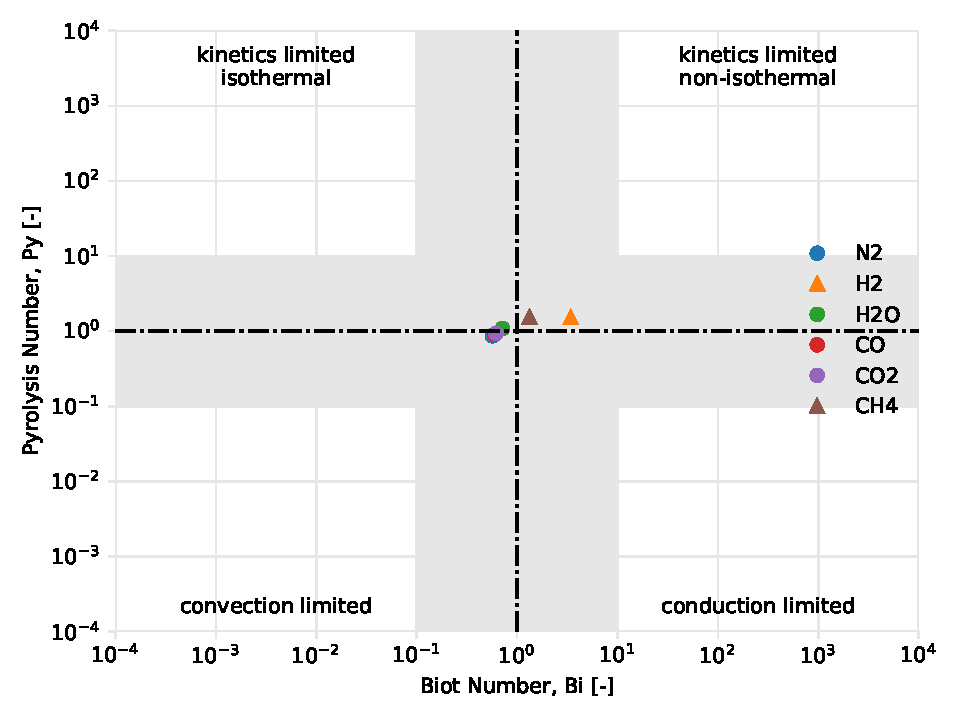
\includegraphics[width=0.8\textwidth]{figures/biot-pyro-gases.pdf}
    \caption{Comparison of carrier gas effects on pyrolysis regime for a 369.4 $\mu$m biomass particle.}
    \label{fig:biot-pyro-gases}
\end{figure}

\begin{figure}[H]
    \centering
    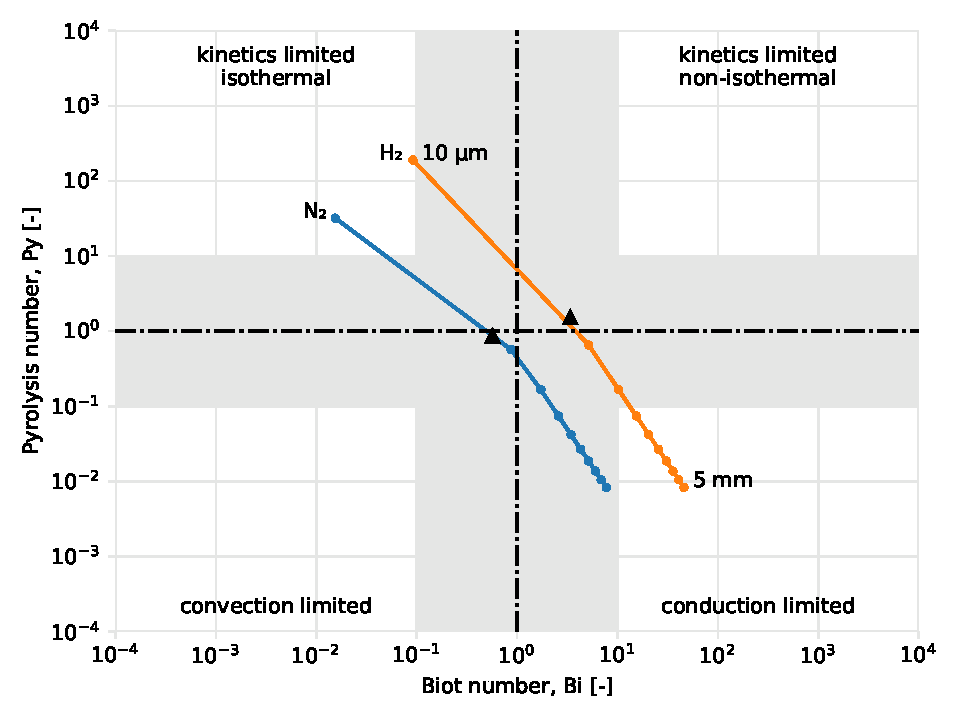
\includegraphics[width=0.8\textwidth]{figures/biot-pyro-diams.pdf}
    \caption{Comparison of nitrogen and hydrogen gas effects for biomass particles ranging from 10$\mu$m to 5 mm in diameter. Triangle markers symbolize 369.4 $\mu$m biomass particle diameter.}
    \label{fig:biot-pyro-diams}
\end{figure}

% ----------------------------------------------------------------------------

\subsection{CFD-DEM validation}

The predicted yield of pyrolysis products (bio-oil, light gas, and biochar) was validated against experimental data reported by [XXX]. In their experimental work, [XXX] carried out biomass pyrolysis in the same NREL 2FBR fast pyrolysis system that is modeled and simulated in this research. Additionally, the process variables used in the experimental work are consistent with those implemented for the N$_2$ and H$_2$ cases in this research. Figure \ref{fig:cfd-validation} shows that the predicted yields of pyrolysis products closely follow the experimental data with absolute deviation ranging between 1\% and 6\%. The largest observed deviations occur in the prediction of bio-oil and are attributed to the non-closure of mass balance for the experimental data. The reported mass closure for the experimental data was about 94\%. A mass-proportional adjustment of the experimental data to enforce 100\% mass closure decreases the absolute deviation of bio-oil prediction to about 2\% or less.

From a qualitative point of view, the implemented CFD-DEM simulation in this research was able to acceptably predict the increase in light gas yield and decrease in biochar yield when fluidizing gas was changed from N$_2$ to H$_2$, as seen in the experimental data. Predicted bio-oil yield slightly increased when fluidizing gas was changed from N$_2$ to H$_2$, contrary to experimental data showing a slight decrease. The relative change in bio-oil yield between N$_2$ to H$_2$ was however quite small for both experimental data (2\%) and CFD-DEM prediction (-1\%).

These results demonstrate that the CFD-DEM model implemented in this research is capable of realistically simulating the characteristic effects of fluidizing gas on the performance of lignocellulosic biomass pyrolysis.

\begin{figure}[H]
    \centering
    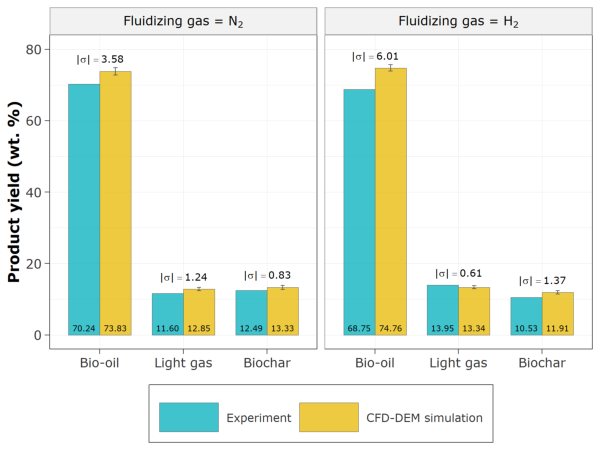
\includegraphics[width=0.8\textwidth]{figures/cfd-validation.pdf}
    \caption{CFD-DEM simulation validation against experimental data. Product yields are calculated on a biomass basis. Deviation between experiment and simulation given by $\sigma$.}
    \label{fig:cfd-validation}
\end{figure}

% ----------------------------------------------------------------------------

\subsection{Fluidizing gas effect on pyrolysis performance with constant flowrate}

Figure \ref{fig:cfd-press-temp} presents the volume-time averaged pressure drop and temperature along the height of the fluidized bed reactor. The different fluidizing gases considered in this research demonstrated similar effects on the pressure drop profile along the reactor height. Overall, the averaged bed height – as evidenced by the inflection point on the pressure drop curve – was about 0.14 m, regardless of fluidized gas. Similarly, the total pressure drop across the reactor was consistently about 1440 Pa for all fluidizing gases and mixtures. The volume-time averaged gas temperature ranged between 495$^\circ$C and 500$^\circ$C, depending on position along the reactor height and fluidizing gas. Gas temperature generally dipped around the biomass inlet and at the dense-bed/dilute- phase interface. The most noticeable trend in gas temperature occurs in the dilute-phase, with increasing gas temperature along the height of the reactor. Also noteworthy is the fact that gas temperature in the dilute-phase was highest when H$_2$ was used as fluidizing gas. This observation is attributable to the large difference in the thermal conductivity of H$_2$ and the other fluidizing gases (Figure XXX). The impact of the difference in the thermal conductivity of fluidizing gases is also evident in the average particle temperature and mass loss profile (Figure \ref{fig:cfd-particle}). When H$_2$ was used as fluidizing gas, biomass particles experienced significantly higher heating rate, and consequently higher mass loss rate, compared to when other fluidizing gases were used. Biomass heating and mass loss rate follow the order: H$_2$ $>$ CH$_4$ $>$ H$_2$O $>$ CO$_2$ $>$ N$_2$ + CO$_2$ $>$ N$_2$ $>$ N$_2$ + CO $>$ CO, irrespective of the initial size of the biomass particle.

Furthermore, it was observed that tar conversion reactions (Reactions 4 and 5) slightly changed among fluidizing gas used, with the lowest being N$_2$ and the highest being H$_2$ (Figure \ref{fig:cfd-biooil}). This observation explains the reason why despite H$_2$ yielded the highest particle heating and mass loss rate (Figure \ref{fig:cfd-particle}), and one of the longest residence times (Figure \ref{fig:cfd-particle-time}), its bio-oil yield relative to biomass flow rate is negligibly different from the bio-oil yield with other fluidizing gases, especially N$_2$. Nevertheless, the fact that we found that fluidizing gas can notably increase biomass heating and mass loss rate (pyrolysis conversion rate) suggest potential process intensification implication because increased heating and pyrolysis rate represents a system where pyrolysis can be completed at an increased rate and consequently offering increased system throughput. Our finding suggests that, at the least, fluidizing gas with produced light gases can be recirculated as fluidizing gas without detrimental consequences on pyrolysis performance.


\begin{figure}[H]
    \begin{subfigure}{0.55\textwidth}
        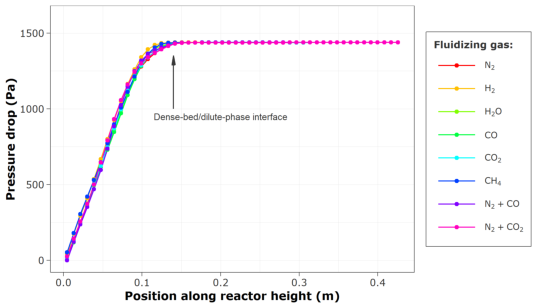
\includegraphics[width=\textwidth]{figures/cfd-pressure.pdf}
    \end{subfigure}
    \begin{subfigure}{0.45\textwidth}
        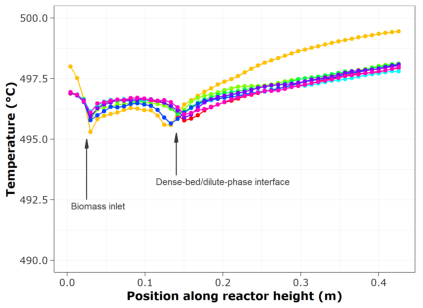
\includegraphics[width=\textwidth]{figures/cfd-temperature.pdf}
    \end{subfigure}
    \caption{Time-averaged distribution of gas phase pressure drop (left) and temperature (right) along the reactor height.}
    \label{fig:cfd-press-temp}
\end{figure}

\begin{figure}[H]
    \begin{subfigure}{0.5\textwidth}
        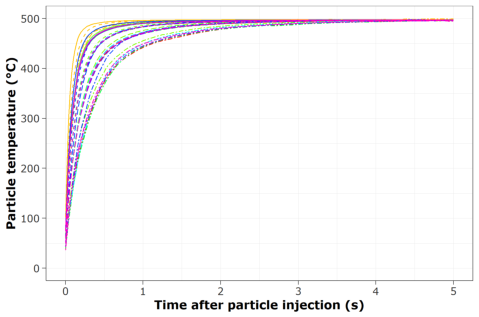
\includegraphics[width=\textwidth]{figures/cfd-particle-temp.pdf}
    \end{subfigure}
    \begin{subfigure}{0.5\textwidth}
        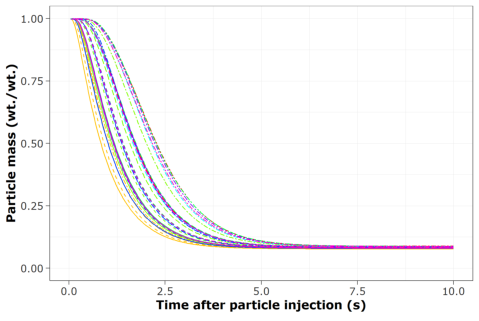
\includegraphics[width=\textwidth]{figures/cfd-particle-mass.pdf}
    \end{subfigure}
    \begin{subfigure}{\textwidth}
        \centering
        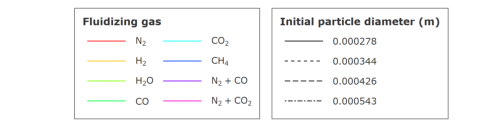
\includegraphics[width=0.6\textwidth]{figures/cfd-particle-legend.pdf}
    \end{subfigure}
    \caption{Average particle temperature (left) and mass loss (right) profile during pyrolysis. Line color discriminates among fluidizing gas, whereas line type discriminates among initial particle diameter.}
    \label{fig:cfd-particle}
\end{figure}

\begin{figure}[H]
    \centering
    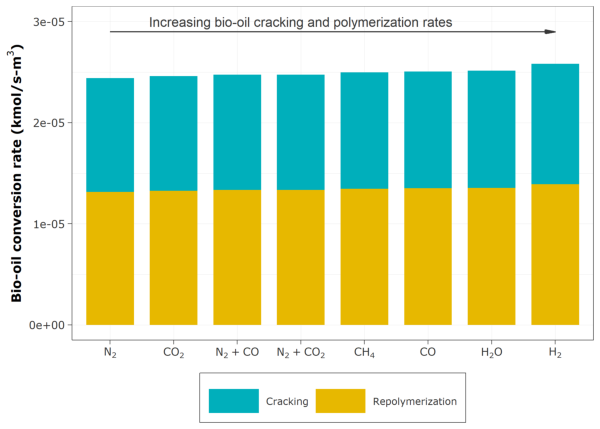
\includegraphics[width=0.8\textwidth]{figures/cfd-biooil.pdf}
    \caption{Time-average bio-oil cracking and polymerization rates.}
    \label{fig:cfd-biooil}
\end{figure}

\begin{figure}[H]
    \centering
    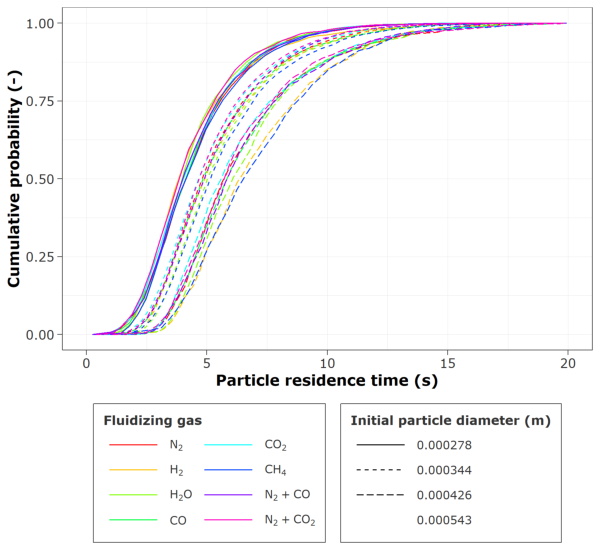
\includegraphics[width=0.8\textwidth]{figures/cfd-particle-time.pdf}
    \caption{Cumulative particle residence time distribution as affected by fluidizing gas and initial particle diameter.}
    \label{fig:cfd-particle-time}
\end{figure}

\begin{figure}[H]
    \centering
    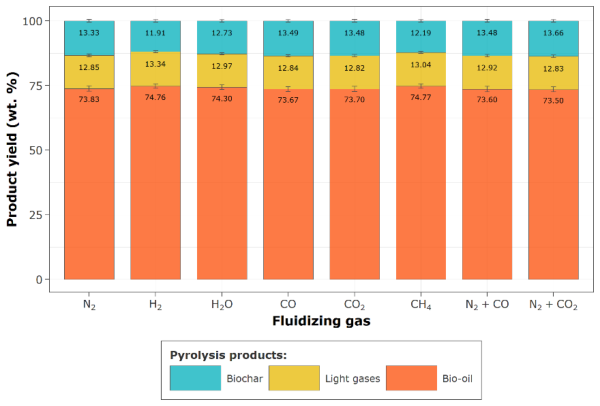
\includegraphics[width=0.8\textwidth]{figures/cfd-yields.pdf}
    \caption{Pyrolysis product distribution as affected by fluidizing gas. Product yields are calculated on a biomass basis.}
    \label{fig:cfd-yields}
\end{figure}

% ----------------------------------------------------------------------------

\subsection{Fluidizing gas effect on pyrolysis performance with constant \texorpdfstring{U/U$_\text{mf}$}{U/Umf}}

As discussed above, the value of U$_\text{s}$/U$_\text{mf}$ varies for each fluidizing gas composition when the flowrate is kept constant. As a result, the dynamic behavior of the bed, which U$_\text{s}$/U$_\text{mf}$ characterizes, varies with the gas composition. These differences are most pronounced between N$_2$ and H$_2$ which have U$_\text{s}$/U$_\text{mf}$ values of ~3.0 and ~1.5, respectively, when U$_\text{s}$ remains constant. To investigate the effect of gas properties on pyrolysis yields, the mass fraction of H$_2$ was varied between 0 and 1 (with the N$_2$ as the remaining fraction) while maintaining a constant U$_\text{s}$/U$_\text{mf}$ = 2.99. Figure \ref{fig:cfd-constuumf-particle-temp-density} shows the average particle temperature and mass as a function of time after injection into the reactor for each particle size in both N$_{2}$ and H$_{2}$ fluiding gas streams. Here it can be seen, as for the constant U$_\text{s}$ case, the larger heat transfer coefficient associated with the H$_2$ fluidizing gas (h$_\text{H2}$ = 2224.3, h$_\text{N2}$ = 368.5 W/m$^2$K) result in greater rates of heat transfer and mass loss. Additionally, the nearly identical time distributions of the particle temperature and mass for H$_2$ with constant U$_\text{s}$ and U$_\text{s}$/U$_\text{mf}$ indicates that total heat transfer to a particle in bubbling fluidized bed is independent of the gas velocity. This is consistent with previous results that while convection increases with gas velocity, this increase is offset by decreases in conduction between solids in the bed \cite{Collier-2004,zhou2009particle}.

\begin{figure}[H]
    \centering
    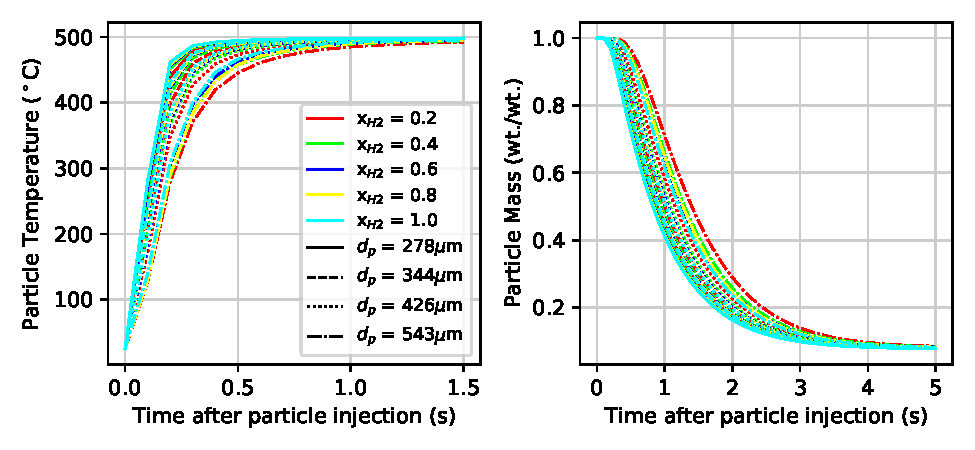
\includegraphics[width=\textwidth]{figures/cfd-constuumf-particle-temp-density.pdf}
    \caption{Average particle temperature (left) and density (right) as a function of residence time in reactor for N$_2$ and H$_2$ carrier gasses. For H$_2$ carrier gas, results with both constant U$_\text{s}$ and U$_\text{s}$/U$_\text{mf}$ are provided.}
    \label{fig:cfd-constuumf-particle-temp-density}
\end{figure}

At the reactor conditions and particle sizes investigated, the gas velocities are insufficient for biomass particles to elutriate from the reactor at their initial density. Therefore, the particle remains in the reactor until its density is sufficiently reduced from pyrolysis. This can be seen in Figure \ref{fig:cfd-constuumf-terminal-vel}, which contains the normalized terminal velocities, U$_\text{t}$/U$_\text{s}$, of each biomass particle size for N$_2$ and H$_2$ (both constant U$_\text{s}$ and U$_\text{s}$/U$_\text{mf}$) fluidizing gases as a function of particle density. For the N$_2$ fluidizing gas, the maximum densities at which U$_\text{s}$ $>$ U$_\text{t}$ are approximately 300, 200, 140 and 90 kg/m$^3$ for particle sizes of 278, 344, 426 and 543 $\mu$m, respectively. These maximum densities decrease to 150, 100, 65 and 40 kg/m$^3$ for H$_2$ at the same gas velocities, but are similar when the flows are increased to maintain a constant U$_\text{s}$/U$_\text{mf}$. This suggests the residence time of the particles is a function of both the terminal velocity of the particles for the given gas mixture, and the rate of heat transfer to the particles, which defines the rate of mass loss from pyrolysis. The result of this can be seen in Figure \ref{fig:cfd-constuumf-rtd}, which contains the average residence time for each particle diameter plotted against the H$_2$ mass fraction in the fluidizing gas. For increasing x$_\text{H2}$ and constant U$_\text{s}$/U$_\text{mf}$, the increasing heat transfer rates result in particles reaching densities necessary for elutriation faster. This, coupled with a nearly constant U$_\text{t}$/U$_\text{s}$, results in the average particle residence time decreasing as H$_2$ x$_\text{H2}$ increases, with the average for all biomass particles decreasing from 5.23s at x$_\text{H2}$ = 0 to 4.64s at x$_\text{H2}$ = 1. For constant U$_\text{s}$, the increased heat transfer rate of H$_2$ are offset by the higher normalized terminal velocity, resulting in the average particle residence time decreasing only ~2.4\% compared to those of the N$_2$ fluidizing gas.

\begin{figure}[H]
    \centering
    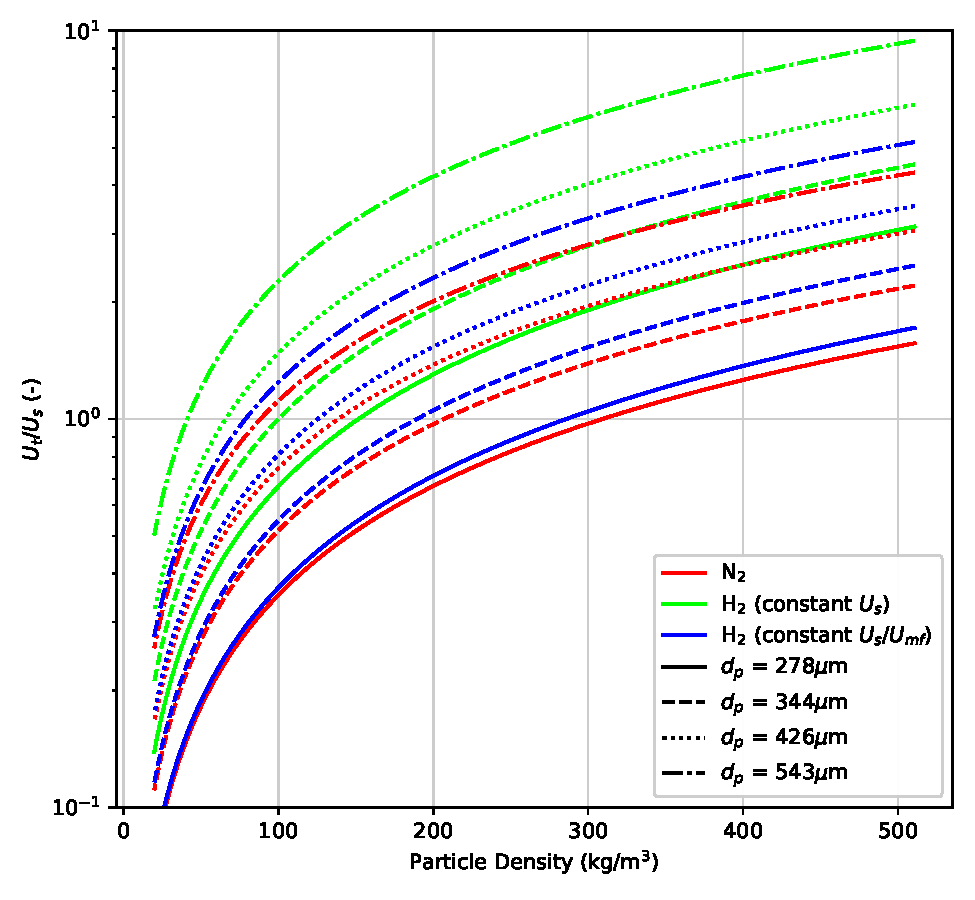
\includegraphics[width=0.8\textwidth]{figures/cfd-constuumf-terminal-vel.pdf}
    \caption{Terminal velocity of each biomass particle size normalized by superficial gas velocity as a function of particle density for N$_2$ and H$_2$ carrier gasses. For H$_2$ carrier gas, results with both constant U$_\text{s}$ and U$_\text{s}$/U$_\text{mf}$ are provided.}
    \label{fig:cfd-constuumf-terminal-vel}
\end{figure}

\begin{figure}[H]
    \centering
    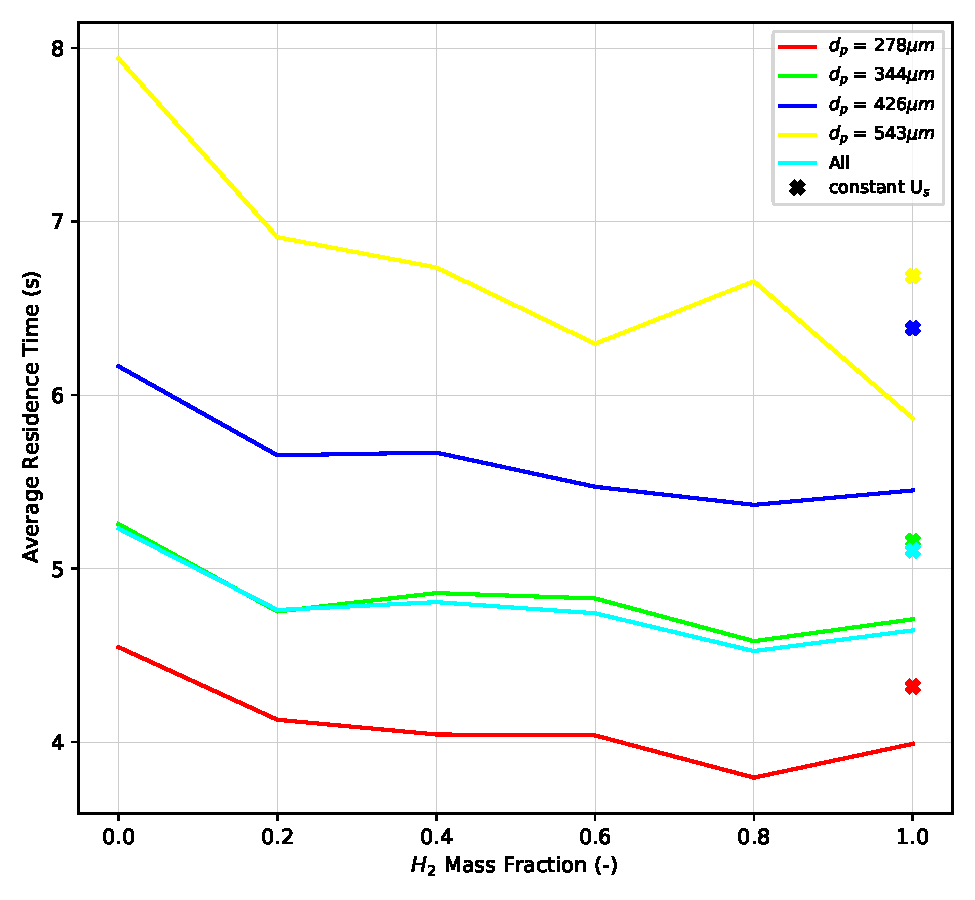
\includegraphics[width=0.8\textwidth]{figures/cfd-constuumf-rtd.pdf}
    \caption{Average particle residence time as a function of H$_2$ mass fraction in fluidizing gas at constant U$_\text{s}$/U$_\text{mf}$. Average residence times for H$_2$ fluidizing gas with constant U$_\text{s}$ indicated by markers in the plot.}
    \label{fig:cfd-constuumf-rtd}
\end{figure}

The effect of maintaining a constant U$_\text{s}$/U$_\text{mf}$ while increasing the mass fraction of H$_2$ in the fluidizing gas can be seen in Figure \ref{fig:cfd-constuumf-yields}, which contains plots of the product yields as well as the fraction of biomass converted for each gas composition and particle size. For d$_\text{p} >= 344$ $\mu$m, the fraction of biomass converted remains nearly constant for each H$_2$ mass fraction, while for 278 $\mu$m, the fraction decreased slightly, a result of the increased gas velocities. For all particle sizes, the yields of light gasses and char decreased with increasing H$_2$ mass fraction with averages decreasing from 12.8\% to 8.38\% and 11.1\% to 9.67\%, respectively. These decreases in the char and light gas yields are accompanied by increases in the bio-oil yields, with the average increasing from 73.8\% in N$_2$ to 79.5\% in H$_2$. For 278 $\mu$m diameter particles, the bio-oil yield initially increased with H$_2$ mass fraction before leveling off between x$_\text{H2} = 0.8$ and 1.0, which resulted from the decreasing fraction of biomass being pyrolyzed before exiting the reactor. The increased yields in bio-oil for increased H$_2$ mass fractions results from the low density of H$_2$ allowing for higher gas velocities while maintaining similar particle residence times. The similar residence times ensure the most of the biomass is converted to its pyrolysis products. With the higher gas velocities, the oil being produced is removed faster, reducing the amount lost to secondary reactions converting it to char (repolymerization) and light gas (cracking). This can be seen in Figure \ref{fig:cfd-constuumf-reaction-rates} which shows the time and volume averaged cracking and repolymerization reaction rates in the reactor for each H$_2$ mass fraction. While maintaining a constant gas velocity when switching the fluidizing gas from N$_2$ to H$_2$ results in a slight increase in both secondary reactions, increasing the gas flowrate to maintain a constant U$_\text{s}$/U$_\text{mf}$ leads to decreases of 35.8\% and 71.3\% for the polymerization and cracking reaction rates, respectively. This leads to the increased bio-oil production and subsequent decrease in light gas and char production when using H$_2$ as the fluidizing gas.

\begin{figure}[H]
    \centering
    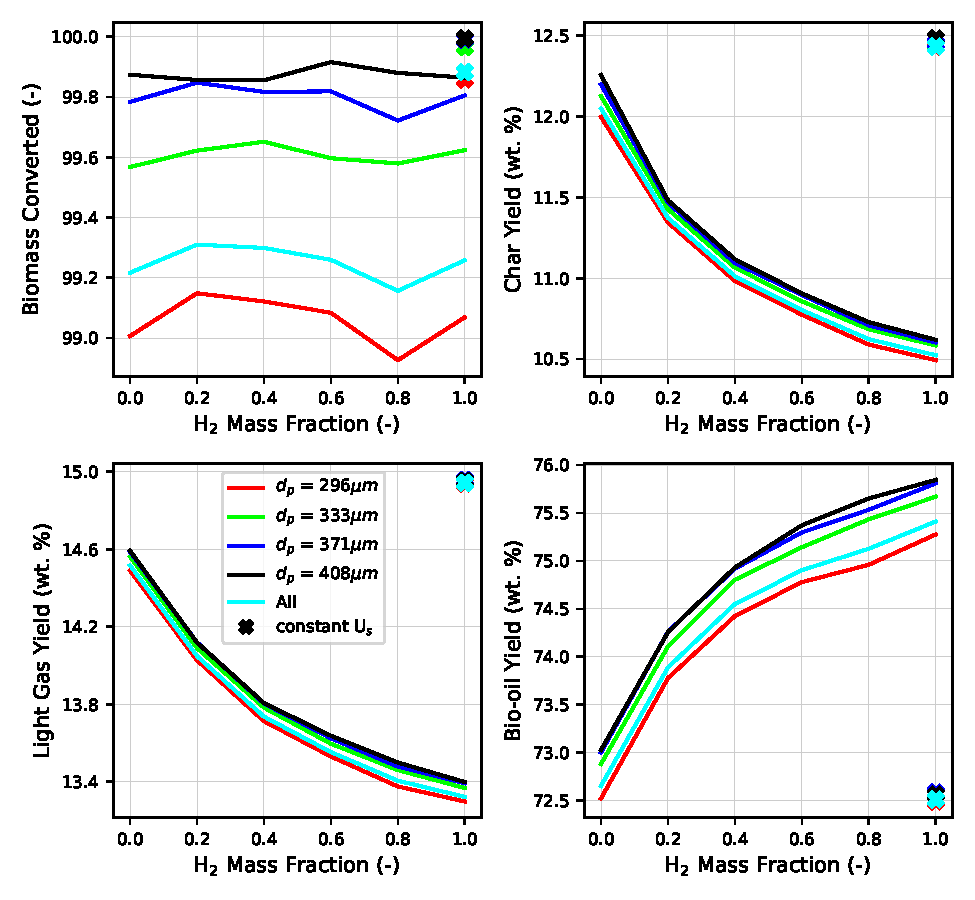
\includegraphics[width=\textwidth]{figures/cfd-constuumf-yields.pdf}
    \caption{Fraction of biomass converted and product yields as a function of H$_2$ mass fraction at constant U$_\text{s}$/U$_\text{mf}$. Biomass converted and product yields for H$_2$ fluidizing gas with constant U$_\text{s}$ indicated by markers in the plot.}
    \label{fig:cfd-constuumf-yields}
\end{figure}

\begin{figure}[H]
    \centering
    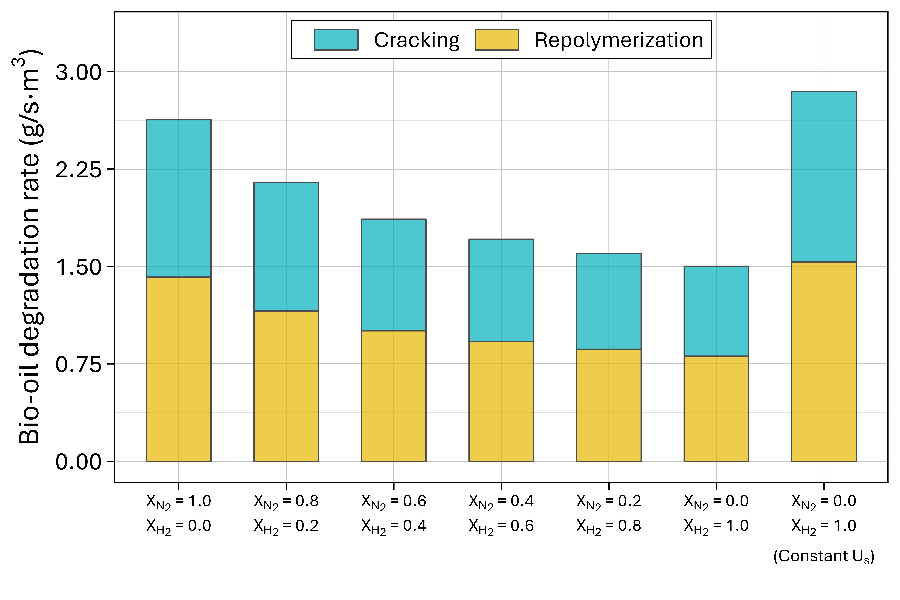
\includegraphics[width=0.8\textwidth]{figures/cfd-constuumf-reaction-rates.pdf}
    \caption{Volume and time averaged secondary reaction rates as a function of H$_2$ mass fraction at constant U$_\text{s}$/U$_\text{mf}$. Reaction rates with H$_2$ fluidizing gas and constant U$_\text{s}$ included for comparison.}
    \label{fig:cfd-constuumf-reaction-rates}
\end{figure}
